\documentclass[usenames,dvipsnames]{beamer}

  \usepackage{amssymb}
  \usepackage[utf8x]{inputenc}
  \usepackage{tikz}
  \usetikzlibrary{calc}
  \usetikzlibrary{shapes.callouts}
  \usetikzlibrary{patterns}

  \usepackage{varwidth}

  \usepackage{color}
  \definecolor{keywordcolor}{rgb}{0.7, 0.1, 0.1}   % red
  \definecolor{commentcolor}{rgb}{0.4, 0.4, 0.4}   % grey
  \definecolor{symbolcolor}{rgb}{0.0, 0.1, 0.6}    % blue
  \definecolor{sortcolor}{rgb}{0.1, 0.5, 0.1}      % green

  \usepackage{listings}
  \def\lstlanguagefiles{lstlean.tex}
  \lstset{language=lean}

  \usecolortheme[RGB={0,137,207}]{structure}
  \setbeamertemplate{navigation symbols}{}

  \title{Metaprogramming in Lean}
  \author{Johannes Hölzl \\ 
\includegraphics{vulogo.png}}
  \date{Hanoi FABS Summer School 2018}

  \newcommand{\kw}[1]{{\color{green!33!black}\ensuremath{\mathtt{#1}}}}
  \newcommand{\ident}[1]{{\color{blue!33!black}\ensuremath{\mathtt{#1}}}}
  \newcommand{\sect}[1]{\begin{frame}
  \begin{center} \Huge{\usebeamercolor[fg]{structure} #1} \end{center}
  \end{frame}
  }

  \tikzstyle{every picture}+=[remember picture]
\begin{document}

\maketitle

\begin{frame}{Metaprogramming: Extend Lean using Lean}
  \begin{itemize}
    \item Writing proofs is not only hard but also time consuming

    \item Tactics help us to construct proofs

    \item Lean is implemented in C++, \\
      we don't want to write C++ code

    \item \textbf{Solution:} Implement Tactics by writing Lean code

    \item Use Lean as functional programming language

    \item \url{https://leanprover.github.io/programming_in_lean/}

  \end{itemize}
\end{frame}

\begin{frame}{Architecture}
  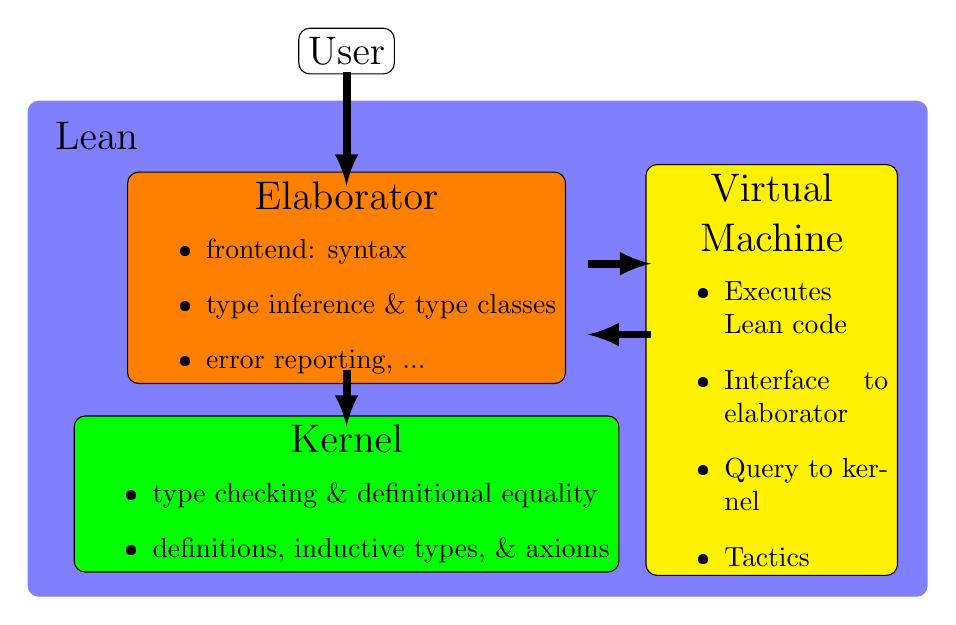
\begin{tikzpicture}[scale=0.9]
    \fill [rounded corners, blue!50!white] (-4.5, -1.7) rectangle (8.2, 5.3) ;
    \node at (-3.5, 4.8) { { \Large Lean } } ;
    \node at (0, 6) [draw, rounded corners] { \Large User };
    \node at (0, 2.8) [draw, rounded corners, fill=orange] {
        \begin{varwidth}{6cm}
        \begin{center} \Large Elaborator \end{center}\vskip -0.5cm
        \begin{itemize}
          \item frontend: syntax
          \item type inference \& type classes
          \item error reporting, ...
        \end{itemize}
      \end{varwidth}
    };
    \node at (0, -0.25) [draw, rounded corners, fill=green] {
        \begin{varwidth}{6.8cm}
        \begin{center} \Large Kernel \end{center}\vskip -0.5cm
        \begin{itemize}
          \item type checking \& definitional equality
          \item definitions, inductive types, \& axioms
        \end{itemize}
      \end{varwidth}
    };
    \node at (6, 1.5) [draw, rounded corners, fill=yellow] {
      \begin{varwidth}{3cm}
      \begin{center} \Large Virtual Machine \end{center}\vskip -0.5cm
      \begin{itemize}
        \item Executes Lean code
        \item Interface to elaborator
        \item Query to kernel
        \item Tactics
      \end{itemize}
    \end{varwidth}
    } ;
    \draw[-latex,line width=1mm] (0, 5.7) -- (0, 4.1);
    \draw[-latex,line width=1mm] (3.4, 3) -- (4.3, 3);
    \draw[-latex,line width=1mm] (4.3, 2) -- (3.4, 2);
    \draw[-latex,line width=1mm] (0, 1.5) -- (0, 0.7);
  \end{tikzpicture}

\end{frame}

\begin{frame}{Definitions in Lean}
  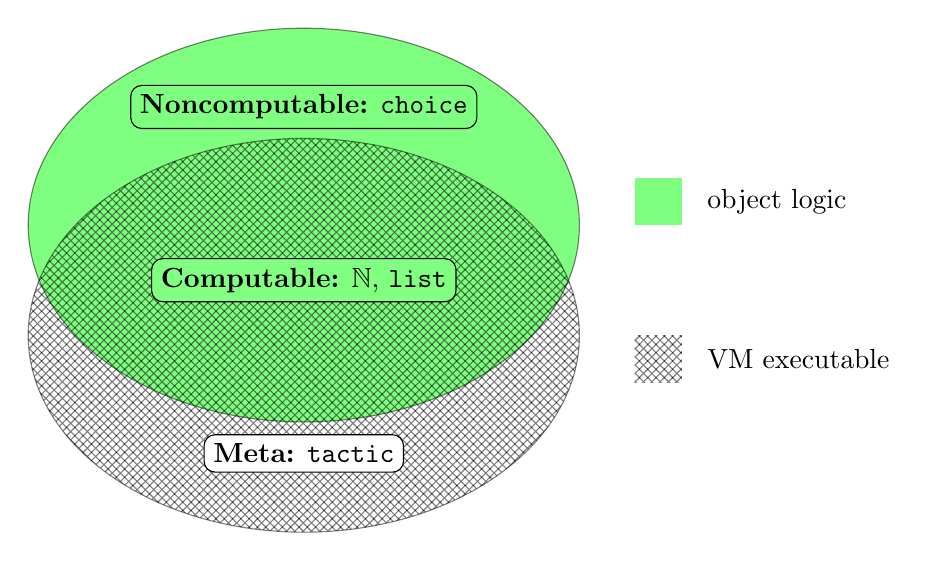
\begin{tikzpicture}
    \draw[opacity = 0.5, fill=green] (0,  0.7) ellipse [x radius=3.5cm, y radius=2.5cm];
    \draw[opacity = 0.5, pattern=crosshatch] (0, -0.7) ellipse [x radius=3.5cm, y radius=2.5cm];
    \node [draw, rounded corners] at (0, 2.2) { \textbf{Noncomputable:} \texttt{choice} };
    \node [fill=green!50!white, rounded corners, draw] at (0, 0) { \textbf{Computable:} $\mathbb{N}$, \texttt{list} };
    \node [fill=white, rounded corners, draw] at (0, -2.2) { \textbf{Meta:} \texttt{tactic} };
    \fill [opacity = 0.5, fill=green] (4.2, 0.7) rectangle (4.8, 1.3);
    \node at (5, 1) [right] {object logic};
    \fill [opacity = 0.5, pattern=crosshatch] (4.2, -0.7) rectangle (4.8, -1.3);
    \node at (5, -1) [right] {VM executable};
  \end{tikzpicture}

\end{frame}

\begin{frame}{What is a Tactic?}
  \begin{itemize}
    \item Basic idea: $\texttt{a\_tactic} : \texttt{expr} \rightarrow \texttt{expr}$
    \begin{description}
      \item[input] the target as proposition (or type)
      \item[result] is a proof (inhabiting term) of the target
    \end{description}
    \item Tactics can fail
    \item Tactics can leave holes in the term
    \item Tactics need access to: local context, attributes, declaration, options, \ldots
    \item We want a framework to construct tactics
  \end{itemize}

\end{frame}

\begin{frame}[fragile]{How is Lean represented in Lean?}
  \begin{description}
    \item[\texttt{name}] Hierarchical names
    \item[\texttt{level}] Represents universe levels as datastructure
    \item[\texttt{expr}] Represents expressions as datastructure
  \end{description}
  \begin{lstlisting}
    meta inductive expr
    | var | sort | const | app | lam | pi | elet
    | macro | mvar | local_const
    \end{lstlisting}
\end{frame}


\end{document}